\subsection{Results}
\label{subsec:cuda:results}

\todorev{Last revised on Sun, July 1 at 00:27 by pfac}

Results for the CUDA implementations are here presented in the form of speedups, relatively to the original raw version of \polu (see \cref{sec:env,sec:method} for details on the environmental setup and methodology used, respectively).
Results were measured by comparing both the first, more naive CUDA implementation, and the last implementation, with better kernels and the division removed from \update kernel.
Some intermediate implementations were also created, since optimizations were aggregated by each new kernel version created, but only the final results of the optimizations are shown in \cref{fig:cuda:results}.

\begin{figure}[!htp]
	\centering
	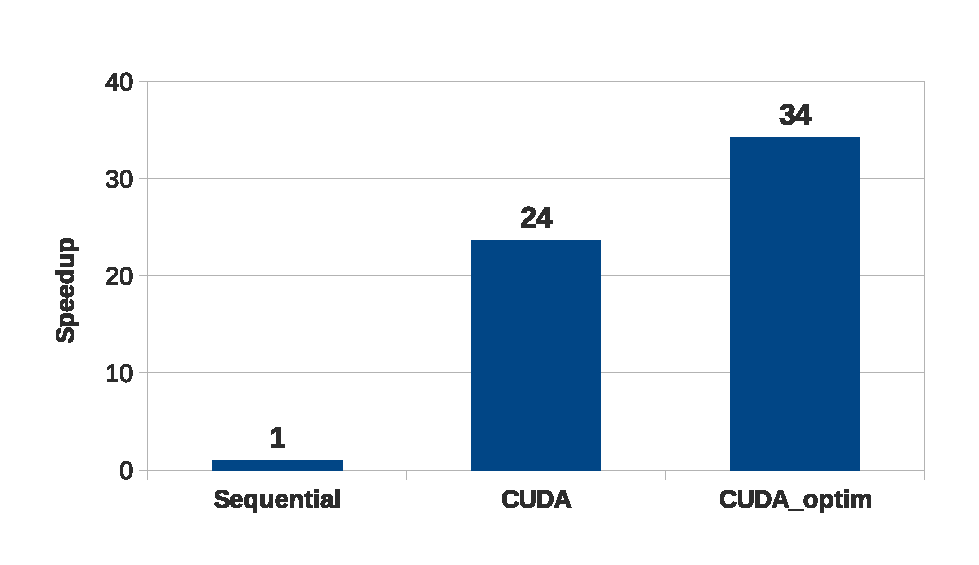
\includegraphics[width=\columnwidth]{graph_comparison_cuda}
	\caption{CUDA implementation speedups}
	\label{fig:cuda:results}
\end{figure}

The initial CUDA version already showed significant performance gains, almost matching the best speedup achieved with the OpenMP implementation in \cref{sec:omp}.
Optimizations were able to boost this speedup even further, achieving a total speedup of 34, the best one in this project.

However, the gain against the OpenMP version is not as large as previously expected, since this problem seemed extremely well suited to a massively parallel approach, like the one employed by CUDA.
This is a result of the limited test case size, which was generated using a conversion utility provided with \polu, that converts \texttt{gmsh} output to a XML file readable by \polu.
This utility was not subject to optimizations or parallelization, but uses an algorithm in the order of $\Theta(N^3)$, making the generation of larger test cases impossible due to time limitations.
The test cases available, which only go up to 62MB, still do not reach the maximum capacity of the GPU, which may benefit from the addition of even more threads.

Given the chance to test this theory, this could show much greater scalability for the CUDA implementation.
